\documentclass[9pt,twocolumn,twoside,lineno]{pnas-new}
% Use the lineno option to display guide line numbers if required.

\templatetype{pnasresearcharticle} % Choose template 
% {pnasresearcharticle} = Template for a two-column research article
% {pnasmathematics} %= Template for a one-column mathematics article
% {pnasinvited} %= Template for a PNAS invited submission

\title{Metaphor and Linguistic Creativity:\\ Pragmatic Reasoning with Distributional Semantics}

% Use letters for affiliations, numbers to show equal authorship (if applicable) and to indicate the corresponding author
\author[a]{Reuben Cohn-Gordon}
\author[b]{Leon Bergen$^{*,}$} 
% \author[a]{Author Three}

\affil[a]{Stanford University}
\affil[b]{University of California San Diego}
% \affil[c]{Affiliation Three}

% Please give the surname of the lead author for the running footer
\leadauthor{Cohn-Gordon} 

% Please add here a significance statement to explain the relevance of your work
\significancestatement{
% Authors must submit a 120-word maximum statement about the significance of their research paper written at a level understandable to an undergraduate educated scientist outside their field of speciality. The primary goal of the Significance Statement is to explain the relevance of the work in broad context to a broad readership. The Significance Statement appears in the paper itself and is required for all research papers.

% Linguistic creativity --- the ability to combine existing representations to create new meanings --- is a distinctive trait of human cognition. Metaphor provides a general vehicle for this creativity: it allows people communicate about one domain, using representations from another. Here, we develop a system for open-domain interpretation of metaphors. Our system integrates world knowledge automatically induced from large text corpora, with reasoning about the social goals of the speaker. The approach provides a general architecture for composing domain-specific knowledge with social reasoning, providing insight into the origins of linguistic creativity.

Linguistic creativity --- the ability to combine existing representations to create new meanings --- is a distinctive trait of human cognition. Metaphor provides a general vehicle for creative transfer and reuse of concepts. Here, we develop a system for open-domain interpretation of metaphor. Our system integrates world knowledge automatically induced from large text corpora, with reasoning about the social goals of the speaker. The approach provides a general architecture for composing semantic knowledge with social reasoning, providing insight into the origins of linguistic creativity.



}

% todos:
	
% 	many many more citations:
% 		nlp metaphor literature
% 		cog sci: see kao paper

% Please include corresponding author, author contribution and author declaration information
\authorcontributions{R.C.G. and L.B. designed the model, planned the experiment, performed analyses, and wrote the manuscript. R.C.G. carried out the experiment.}
% \authordeclaration{Please declare any conflict of interest here.}
% \equalauthors{\textsuperscript{1}A.O.(Author One) and A.T. (Author Two) contributed equally to this work (remove if not applicable).}
\correspondingauthor{\textsuperscript{*}To whom correspondence should be addressed. E-mail: LBergen@ucsd.edu}

% Keywords are not mandatory, but authors are strongly encouraged to provide them. If provided, please include two to five keywords, separated by the pipe symbol, e.g:
\keywords{metaphor $|$ informativity $|$ Bayesian pragmatics $|$ distributional semantics}


\begin{abstract}
Humans create and interpret novel metaphors, like \emph{Time is a thief} or \emph{My lawyer is a shark}, with relative ease, incorporating contextual knowledge to determine which aspects of the predicate (\emph{thief, shark}) are true of the subject (\emph{time, my lawyer}). Here we present a computational theory of metaphor, according to which metaphorical interpretations arise from joint, cooperative reasoning between a speaker and listener. We combine a Bayesian model of this reasoning process with empirically learned \emph{word embeddings} which are used to provide an underlying representation of word meaning. This allows for open-domain interpretation of predicative and adjectival metaphors. We find a significant preference in human judgments for our model over a system which uses word embeddings without a explicit representation of inter-agent reasoning, providing evidence that reasoning about an informative and relevant speaker is key to understanding non-literal language.


% and by doing so interprets a predicative metaphor (of the form ``A is a B''), by identifying the properties of B that are relevant to A. 
% This reasoning process can be modeled probabilistically in the \emph{Rational Speech Acts framework} \cite{frank2012predicting}.
% as a nested inference, where listeners and speakers are Bayesian agents who make inferences about the state of the world and the optimal utterance, respectively.
% However, previous instantiations of these models have required a hand-specified semantics, restricting the generality of the model and the scope of empirical investigation into the effectiveness of pragmatic reasoning for metaphor interpretation.

% We present a method to combine empirically learned word embeddings with a Rational Speech Acts model of metaphor. 


\end{abstract}

\dates{This manuscript was compiled on \today}
\doi{\url{www.pnas.org/cgi/doi/10.1073/pnas.XXXXXXXXXX}}

\newcommand{\Listener}{L}
\newcommand{\QLONE}{\Listener_{{1}}^{{Q}}}

\begin{document}

\maketitle
\thispagestyle{firststyle}
\ifthenelse{\boolean{shortarticle}}{\ifthenelse{\boolean{singlecolumn}}{\abscontentformatted}{\abscontent}}{}


% Note: please start your introduction without including the word ``Introduction'' as a section heading (except for math articles in the Physical Sciences section); this heading is implied in the first paragraphs. 
	% Metaphor is a central case of linguistic creativity, where the combination of words produces a novel meaning, in a context dependent fashion. As such, it... 
Metaphor presents a compelling theoretical challenge for the understanding of meaning in natural language. On hearing (\ref{met:1}) in a context where the subject, Jane, is known to be a journalist, a listener might infer that Jane is not literally a soldier, but rather that she shares certain attributes with soldiers (perhaps determination, endurance, or ruthlessness). 
	% Similarly, on hearing a temper described as \emph{fiery}, a listener might infer that 
	\begin{examples}
	% % \vspace{-1.0em}
	\item Jane is a soldier \label{met:1}
	\end{examples}

The \emph{pragmatic} view of metaphor, proposed by Grice \cite{grice}, takes the meaning conveyed by sentence (\ref{met:1}) to be the result of joint, cooperative reasoning between a speaker and listener. That is, the listener attempts to jointly infer what Jane must be like and what aspects of Jane are plausibly relevant for the speaker. The speaker, in turn, wants to communicate about these aspects of Jane, and chooses the predicate \emph{soldier} over other alternatives.



% Our goal is to evaluate the accuracy of the Gricean view as a model of human cognition, regarding metaphor interpretation. To do so, we construct a model of metaphor which relies on pragmatic reasoning of this form, and elicit human judgments comparing its predictions to a non-pragmatic baseline. 
		% Our goal is to provide evidence towards this view, by 

\paragraph{Interpreting figurative language}
% Previous work in linguistics and cognitive science has modeled this type of pragmatic reasoning in a probabilistic framework \cite{frank2012predicting}.
% In this work, there is a speaker whose goal is to communicate a particular state and who chooses an utterance in order to satisfy this goal, with the listener in mind. A listener then interprets an utterance by inferring the communicative goal which would have led the speaker to choose this utterance. 

% language interpretation in context as the product of joint reasoning between rational agents \cite{frank2012predicting}. 

	% This framework models pragmatic interpretation and production of language via probabilistic models of speakers and listeners, who reason about each other in a nested fashion, with the assumption of cooperativity and a shared semantics.

We build on a previous model of metaphor interpretation \cite{kao}, developed as part of a probabilistic framework for pragmatic reasoning \cite{frank2012predicting}, which uses \emph{projection functions} to determine the dimension of the world that the speaker cares about communicating. In this model, a listener jointly reasons about the state of the world (e.g. what Jane is like) and a projection function, corresponding to the aspect of the world the speaker cares to communicate (e.g. Jane's determination). This listener assumes an informative speaker - one whose choice of utterance maximizes the probability of communicating the state of the world - but only up to a projection which dictates the relevant dimension of the world.

% Kao et al. \citep{kao} extend the framework by introducing a new model, $\QLONE$, which is able to interpret metaphors. 
% Obtaining metaphorical interpretations for utterances like (\ref{met:1}) is within the scope of a formalization of pragmatic reasoning, the \emph{Rational Speech Acts} (RSA) framework \cite{frank2012predicting}. 
	% Pragmatic accounts of metaphor, stemming from \cite{davidson} and \cite{grice}, attempt to derive metaphorical meaning as the inference of a language user reasoning about an expression heard in a given context. For instance, on hearing (\ref{met:1}), a listener infers 

	% Grice suggests that a listener infers that an expression they hear is metaphorical on account of the unlikelihood of its literal interpretation being true, and further infers which elements of the 

	 % Further, the listener reasons 
	% 	fix this: should be: example of key importance:
	% As \cite{shutova} notes, core NLP tasks such as translation often require an understanding of metaphor:
	% 		The train of progress stormed across the country

				% examples only apply if metaphor is conventionalized: otherwise you could just translate the metaphor:

					% possibly not always: John is a shark

	% Accounts of metaphor can be broadly divided on the basis of whether they treat metaphor as a semantic or pragmatic phenomenon. The former camp (e.g. \cite{lakoff}), treats metaphor as a fundamental part of semantic meaning, or even thought. The latter,

	

	% makes empirical validation of the model difficult
	% , because of the bias introduced by the hand-chosen semantics.

	% This precludes a fair test of whether the model succeeds, because of the need for a stipulated (and therefore potentially biased) semantics.
	
% 
	% However, applications of this model have been restricted to cases with a hand-constructed semantics, where the meanings of the predicates in question has to be stipulated.

	% While still a useful proof of concept, 
	% The question therefore remains of whether the central theoretical assumption of the model, that a Gricean process of reasoning about relevance and informativity is a good model of human behavior, as regards metaphor interpretation. 
	This can be used to give an account of predicative metaphors (those of the form \emph{A is a B}) and adjective-noun (AN) metaphors (like \emph{fiery temper}). However, in order to generate predictions from the model, it is necessary to provide a semantics, specifying the literal meaning of each utterance (for example, that \emph{soldier} literally describes an individual who serves in a military). Previous work has hand-constructed these literal interpretations, restricting the scalability of the models, and their applicability to previously unseen metaphors.

	\paragraph{Our contribution} 


	We develop a model of pragmatic reasoning which uses empirically learned word-embeddings \cite{mikolov2013distributed,pennington2014glove} to represent word meanings, obtaining a system capable of interpreting open-domain predicative and adjectival metaphors without the need for hand-specified semantics. 
	This adaptation requires a generalization of projection functions to linear projections in a vector space, and a novel inference algorithm to calculate metaphor interpretations.
	Constructing this system permits what is to our knowledge the first open-domain evaluation of a Bayesian model of pragmatic reasoning.
	Evaluated on human judgments, our model significantly outperforms a baseline which uses a word embedding semantics without explicit pragmatic reasoning. This suggests that the information in word embeddings alone is not sufficient to capture the creativity of metaphorical language, but that an explicit model of pragmatic reasoning is also key.

	% We conduct the first open domain evaluation of 

	% We adapt $\QLONE$ to a setting where the denotations of words are points in an abstract, and empirically determined, vector space. Such \emph{word embedding} spaces are a core NLP tool, and have been shown to represent various notions of semantic similarity via the geometry of the space \cite{pennington2014glove}.
		

	% Adapting the $\QLONE$ model to allow for denotations of this kind requires us to introduce a new semantics, to generalize the notion of a projection to a vector space, where it amounts to a linear projection, and to develop an approximate inference algorithm to calculate the now  

	% By doing so, we obtain a model capable of interpreting arbitrary predicative and adjectival metaphors, without the need for a hand-specified semantics. 
	% This allows us to assess to efficacy of the Gricean view of metaphor (as formalized in $\QLONE$), by evaluating our model on human judgments. In particular, w
			% We take this to be evidence that the Gricean account of metaphor, formalizes as a joint inference over state of the world and 
			% 	blah
			% 		of the speaker, is a good theory of metaphor.


	% Within the paradigm of Bayesian pragmatics\footnote{See \cite{frank2012predicting} for an introduction to the Rational Speech Acts (RSA) model more generally} (\cite{kao}) proposes a model which conducts joint inference over the attributes of a referent and a \emph{question under discussion}. This Bayesian formalization offers not only a way to recognize that metaphorical expressions are not to be interpreted literally, like Grice suggests, but also a way to access the meaning the metaphor \emph{does} convey.

			

	% This Bayesian model offers a natural formalization of the intuitions of earlier pragmaticists and has allowed for rigorous experimental investigation. A further use of RSA in is computational models of semantics and pragmatics; recent work (e.g. \cite{andreas}, \cite{monroe2015learning}) has focused on integrating these Bayesian models with modern advances in computational linguistics.

	% Our contribution to this enterprise focuses on incorporating word vector semantics into RSA. To this end, we implement a model of RSA which has an infinite number of world states, which correspond to points in a word vector space. Furthermore, we implement a more complex variant of RSA (based on the work of \cite{kao}) that involves a notion of QUDs, so that the model reasons about which \emph{aspects} of word meaning are relevant to a given metaphor.

			% , showing that

			% 	computationally 
			% 		blah
			% 			implementations of RSA can model more that scalar implicature
			% 				chris will obviously tear this apart




	% Given the success of word embeddings at a range of linguistic tasks (see \cite{turney2010frequency}), it is natural to wonder whether such embedding spaces can provide a knowledge base for a model of metaphor which is scalable to real world data.

	% Building on the work of (\cite{kao}), we design and implement a distributional Bayesian model of metaphor meaning, which applies RSA to a semantics grounded in pretrained word embeddings. 

	% This model, which we refer to as DistRSA, allows us to generalize the RSA model of metaphor well beyond the hand-constructed examples which previous pragmatic models require. We apply our model to two task, which we view as crucial to the computational processing of metaphorical language: metaphor understanding, and metaphor detection.


		% The goal of a speaker is to produce an utterance which informs their interlocutor of the speaker's position in this space, to which end they may employ metaphorical language. For instance, if John is a ruthless businessman, then the sentence ``John is a shark.'' should enable the listener to infer John's position in the space.
\section{Overview of metaphor}

	Metaphor exists in many syntactic forms \cite{black1954metaphor}, and has been extensively studied in cognitive science \cite{tourangeau1981aptness,roberts1994people,camp2006metaphor}, linguistics \cite{glucksberg1993metaphors,lakoff1993contemporary} and other disciplines \cite{martin1990computational,davidson}.

	% , and generally eludes easy definition. 
	For present purposes, we focus on metaphors involving copular predicates (e.g. \emph{Jane is a soldier}) and AN noun phrases (e.g. \emph{fiery temper}). We refer to the predicated or modified noun (\emph{Jane}, \emph{temper}) as the \emph{target} of the metaphor and the predicate or adjective (\emph{soldier}, \emph{fiery}) as the \emph{source} (see \cite{lakoff1980metaphors} for the more general sense of these terms).

	% We focus on predicative metaphors of the form ``A is a B'' (e.g. ``John is a shark.''), as well as metaphorical modification, e.g ``fiery temper'' or ``golden opportunity''. We further consider the possibility that the meaning of metaphorical phrases such as these can be interpreted as the posterior position of the head noun, after the model observes the modifying adjective.

	For a given metaphor, only certain properties of the target are described by the source, and which these are depend on the metaphor and the context. For instance, (\ref{dog}), said of a sleeping dog, could convey that it is unresponsive, but said of a large alert dog, could convey that it is heavy.

	% For instance, (\ref{bread}) likely conveys that the bread is like a rock with respect to hardness, while (\ref{dog}) likely conveys that the sleeping dog is like a rock with respect to its responsiveness. However, we could also imagine a context in which the dog is very heavy, so that a more natural inference is that it is like a rock with respect to its weight.

	\begin{examples}
	% \item The bread is a rock. \label{bread}
	\item The dog is a rock. \label{dog}
	\end{examples}

	While certain metaphors are conventional - comparing someone to a lion tends to connote bravery - examples like (\ref{dog}) suggest that the interpretation of a metaphor is contextually dependent. The benefit of the pragmatic view of metaphor is the ability to explain this dependence on context, in a way which takes into account an underlying semantics (e.g. the conventional meanings of \emph{dog} and \emph{rock}).
	% requires the listener to reason about the context. It is this contextuality which makes the Gricean account appealing.	
	% Parallel to metaphorical predication, one also finds cases of modification where an adjective modifies a noun in certain regards and not others. Thus, a \emph{fiery temper} shares with fire different properties to a \emph{fiery dish}, and in turn, both differs from a more literal usage, as with a \emph{fiery stove}.
	
	% The first example above is one of literal predication: the granite really is a rock. 
\section{A Bayesian model of metaphor interpretation} \label{rsa}
	
	The Rational Speech Acts framework (RSA) provides an elegant and practical way of formalizing pragmatic reasoning \cite{frank2012predicting}.
	% \footnote{For an interactive introduction, we recommend \url{http://gscontras.github.io/ESSLLI-2016/chapters/1-introduction.html}.}
	In this framework, listeners and speakers are represented as conditional probability distributions. Speakers are represented as distributions over possible utterances given worlds, and listeners as distributions over possible worlds given utterances.
	% Thus, speakers are distributions over possible utterances given worlds, and listeners are distributions over possible worlds given utterances.
	The most basic version of RSA \cite{frank2012predicting} is incapable of interpreting metaphors, due to the strict assumption that the speaker's utterances are literally true. To address this, Kao et al. \cite{kao} propose a model $\QLONE$, shown in (\ref{defl1}), which in turn is defined in terms of $S_1$ (\ref{defs0}) and $L_0$ (\ref{defl0}).

	% RSA works by defining successive levels of speaker and listener recursively. For instance, an informative speaker $S_1$ given a state $w$ chooses the utterance $u$ which maximizes the probability that $L_0$, a listener who interprets utterances literally according only to a semantics,  infers $w$. A pragmatic listener, on hearing some $u$, can then reason about what state $w$ a speaker must have had in mind in order to have said $u$.

	 % which is defined in terms of a semantics $\llbracket\cdot\rrbracket$. 


	% Equation (\ref{defl1}) describes the 

	% We now review the RSA model $\QLONE$ proposed by \cite{kao}, which is capable of interpreting simple metaphors. This is the model 
	% 	our system
	% 		uses, although 
	% 			with a vectorial semantics

	% It is defined in (\ref{defl1}), in terms of speaker model $S_1$, which in turn is defined in terms of a literal listener model $L_0$. 
	% 	This nested architecture is the mechanism by which Gricean reasoning is represented probabilistically.

	% \begin{examples}
	% \item  $L_0(w\vert u) \propto \llbracket u\rrbracket(w)*P_L(w)$ \label{defl0}
	% \end{examples}

	\begin{examples}
	% \item $L_0(w\vert u) = \frac{\llbracket u \rrbracket (w) P_L(w)}{\sum_{w'\in W}\llbracket u \rrbracket (w') P_L(w')} $ \label{defl0}
	\item $L_0(w\vert u) \propto \llbracket u \rrbracket (w)\cdot P_L(w)$ \label{defl0}
	\item $S_1(u\vert w,q) \propto \sum_{w'} \delta_{q(w)=q(w')} \cdot L_0(w'\vert u)$ \label{defs0}
	\item $\QLONE(w,q\vert u) \propto S_1(u\vert q,w)\cdot P_L(w)\cdot P_{L_Q}(q)$ \label{defl1}
	\end{examples}


	\paragraph{The literal listener} $L_0$ represents a model of a listener that, given an utterance $u\in U$, updates their belief about the world $w\in W$ by filtering out all worlds that are semantically incompatible with $u$. The term $\llbracket\cdot\rrbracket$ is a function $U\to(W\to\{0, 1\})$, representing the semantics of the language. $P_L(w)$ is the prior probability of world $w$. 


	\paragraph{Projections} 
	Functions $q\in Q$ formalize the notion of picking a particular \emph{aspect} or \emph{dimension} of $w$. Formally, they are functions $W \to D$, for some set $D$.
	% A simple example is as follows: suppose that $W=AxB$, where $A = \{\textrm{Jane is hardworking}, \textrm{Jane is lazy}\}$ and $B = \{\textrm{Jane owns a gun}, \textrm{Jane doesn't own a gun}\}$, so that each $w\in W$ is a tuple $(a,b)$ for $a\in A, b\in B$. Then the two projections, which we could call $q_{\mathit{work-ethic}}$ and $q_{\mathit{gun-ownership}}$, are defined as $\lambda (x,y): x$ and $\lambda (x,y): y$ respectively. A third trivial projection is simply the identity function.
	

	\paragraph{The informative speaker} $S_1$ has a state $w$ they want to communicate to the listener $L_0$, and prefers utterances $u$ which maximize the probability that $L_0$ assigns to $w$, up to the dimension of $w$ specified by $q$. $\delta_{a=b}$ is an indicator function, and is equal to 1 if $a=b$, and equal to 0 otherwise. If $q$ is the identity function, then $S_1(u|w) \propto L_0(w|u)$, and $S_1$ is thus a model of a speaker who prefers to choose the most informative utterance available. 
	% For example, if trying to communicate state $w$, $S_1$ will prefer an utterance $u$ which is compatible under the semantics with only $w$, over an utterance $u'$ which is compatible with both $w$ and $w'$. 
	
	\paragraph{The pragmatic listener} The full model, $\QLONE$, hears an utterance $u$, and jointly infers values for $w$ and $q$ by reasoning about $S_1$. The key dynamic is that the listener may hear an utterance $u$ and infer a pair $(w,q)$ where $u$ is semantically incompatible with $w$ (i.e. $\llbracket u\rrbracket(w)=0$); this will occur when $u$ conveys effectively some feature of world $w$ as determined by $q$. $P_{L_Q}(q)$ is the prior probability of projection $q$.

	$\QLONE$ functions as a model of metaphor interpretation. For instance, using the metaphor in (\ref{johnshark}), the listener infers both a state $w$ (representing what John is like) and a feature $q$ (representing which aspects of John are relevant).

	As an example in a hand-constructed setting, we could take John to be fully characterized by two features, whether he is vicious and whether he is aquatic, so that a state $w$ is a value (true or false) for both of these predicates. The projections $q\in Q$ are then the functions mapping a state to its value on viciousness ($q_{vicious}$) or aquaticness ($q_{aquatic}$) respectively. Further, we assume that \emph{shark} is semantically compatible only with the state in which John is both vicious and aquatic.


	% To this end, they choose a predicate $u$, here \emph{shark}. The goal of the listener on hearing (\ref{johnshark}) is to infer $w$ as well as the \emph{dimension} of $w$ that the speaker cares about.

	\begin{examples}
	\item John is a shark. \label{johnshark}
	\end{examples}

	% AN metaphor interpretation, the focus of our experiment in section \ref{exp}, in the following way.\footnote{Note that an account for predicative metaphors, with a more conventional truth-conditional semantics can be provided in a similar fashion.} 
	% Suppose that the goal of a speaker is to choose an adjective $u$, out of some set $U$, which communicates some modification of the noun (e.g. \emph{temper}). The goal of the listener is then to infer the desired modification of this noun, on hearing an adjective, like \emph{fiery}.
	



		% Suppose that John can be represented by two Boolean values, and that there are two projections, $q_{vicious}$ and $q_{aquatic}$.

		
	% In theory, for larger n-tuples of properties, a projection could map to multiple properties, representing a speaker who wishes to communicate multiple aspects of the state $w$. We return to this point in our concluding discussion.
	
	% The results of $\QLONE$ hearing \emph{shark} are shown in figure \ref{fig:l1barplot}.
	On hearing (\ref{johnshark}), the prior belief that John is not literally an aquatic animal leads $\QLONE$ to conclude that the speaker cares about conveying the viciousness dimension (i.e. has projection $q_{vicious}$), and that John is vicious. See \cite{kao} for quantitative examples.
	% See \emph{Materials and Methods} for quantitative details.

	Importantly, $\QLONE$ can do more than simply using prior knowledge to interpret literally false statements in a flexible way. It is also capable of reasoning about alternative utterances: for instance, suppose we add a third property, \emph{quickness}, so that \emph{shark} is compatible only with the state in which John is quick, aquatic and vicious, and also add a third utterance, \emph{dolphin}, compatible only with John being quick, aquatic and \emph{not} vicious.

	% $(\textrm{vicious}=F, \textrm{non-human}=T, \textrm{quick}=T)$.
	
	In this second example, when $\QLONE$ hears \emph{shark}, it infers that John is more likely vicious than quick. This is because a speaker who wanted to communicate that John is vicious would only be able to use the utterance \emph{shark}, whereas a speaker who wanted to communicate that John is quick would be able to choose between either \emph{shark} or \emph{dolphin}. The utterance \emph{shark} is therefore more likely to have been produced by the speaker trying to communicate John's viciousness.

	
	% on the assumption that it is compatible with only $(\textrm{intense}=T,\textrm{warm}=T)$ are shown in figure \ref{fig:l1barplot}. 

		% Let the set of all properties under consideration be $P$, and call the function $E : U\to P$ take utterances to their corresponding sets.


	% In order to elicit human-like behavior from the model, \citet{kao} use a set of $\sim$100 animals as alternative utterances $u\in U$, and assemble a property set $P$ experimentally. However, the semantics, relating adjectives to properties 
	$\QLONE$ can model AN metaphors in a similar way. For a phrase like \emph{John's fiery temper}, the listener infers the features of John's temper that would explain why the speaker modified it with \emph{fiery}.

	% \begin{figure}
	% \centering
	% 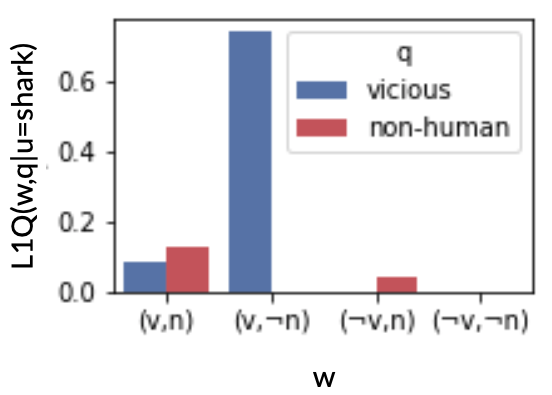
\includegraphics[width=0.4\textwidth]{images/l1posteriorquality.png}
	% % \begin{subfigure}{0.5\textwidth}
	% % % \centering
	% % \end{subfigure}\hfill\begin{subfigure}{0.5\textwidth}
	% % % \centering
	% % 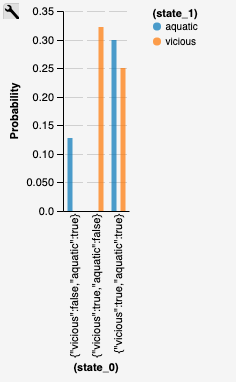
\includegraphics[width=\textwidth]{images/l1posteriorquantity.png}
	% % \end{subfigure}
	% \caption{Figure showing the posterior distribution of $\protect\QLONE$ on hearing \emph{shark}. $v$ and $n$ abbreviate the Boolean variables \emph{vicious} and \emph{non-human} respectively.}
	% \label{fig:l1barplot}
	% \end{figure}

	\section{Distributional Semantics} \label{distmods}

	%From a linguistic corpus, it is possible to obtain a mapping from words to points in a high-dimensional vector space that has the property that semantic similarity of a pair of words $a$ and $b$ corresponds to a metric, such as cosine distance, between the vectors $\overrightarrow{a}$ and $\overrightarrow{b}$.

	\emph{Word embeddings}, or \emph{distributional semantic models}, provide a representation of word meanings that can be learned from large corpora of language data. In these models, word meanings are mapped to points in a high-dimensional vector space, such that words with similar meanings are mapped to nearby points in the space. The embeddings can be obtained either by dimensionality reduction of a word co-occurrence matrix \cite{pennington2014glove} estimated from a corpus, or by extracting the weights of a statistical model \cite{mikolov2013distributed,peters2018deep,devlin2018bert} trained on a separate task. In both cases, word embeddings provide a way to empirically obtain fine grained connotations of lexical items \cite{mikolov2013distributed}, and have been used effectively in a number of NLP tasks \cite{dai2015semi,radford2018improving,socher2013recursive}. 
	% They have also been used to compute vectorial representations of phrases and sentences \cite{socher2013recursive, coecke2010mathematical}.

			% word embeddings appear to encode syntactic and semantic information (\cite{mikolov2013linguistic}, and as such, are useful element in many NLP tasks such as sentiment analysis \cite{socher2013recursive}.

	% (\cite{pennington2014glove}) argues that GloVe vectors exhibit a degree of linear structure, in the sense that for various quadruples of words (A,B,C,D), such that A is to B as C is to D, the corresponding pretrained vectors approximately satisfy the equation $\overrightarrow{\text{A}} - \overrightarrow{\text{B}} = \overrightarrow{\text{C}} - \overrightarrow{\text{D}}$, where $\overrightarrow{\text{A}}$ is the word vector corresponding to the word A. For instance, the nearest word vector by cosine distance to the point ($\overrightarrow{\text{king}}-\overrightarrow{\text{man}}+\overrightarrow{\text{woman}}$) in the Word2Vec embedding space is $\overrightarrow{\text{queen}}$.
	

		

	Metaphor is an obvious candidate for approaches that use distributional semantics: a wide variety of attempts have been made to leverage the information inherent in pre-trained word vectors for the detection, interpretation and paraphrase of metaphor (see \cite{shutova2016design} for an overview of proposed systems).
		% TODO: needs your own citations

	We hypothesize that, while the information in high quality word embeddings captures important aspects of meaning, a cognitively realistic model of metaphor interpretation should also incorporate pragmatic reasoning, of the sort formalized in the RSA framework. We now explain how the $\QLONE$ model described above can be combined with a distributional model of word meaning.

	\section{Bayesian pragmatics with distributional semantics} \label{bayesdist}

	% T$\QLONE$ takes states $w \in W$ to be sets of properties describing the source of the given metaphor, and a semantics to be a function $U\to(W\to\{0, 1\})$.
	% , projections to be surjective functions out of $W$
	% . The semantics maps utterances to functions from worlds to Boolean values, or equivalently, maps a pair $(u,w)$ to $1$ if they are compatible, and $0$ otherwise.

	We now introduce a \emph{vector} interpretation of $\QLONE$. Importantly, this requires no modification to equations (\ref{defl0}-\ref{defl1}). The crucial difference is that our state space $W$ is now not just a set, but a vector space, so that elements $\overrightarrow{w}\in W$ are vectors. A word embedding maps words to vectors ($E : U\to W$).
	% \footnote{We note that this generalization is natural, since the set-theoretic interpretation of $\QLONE$ can be viewed as a special case of the vectorial interpretation, for a vector space over the Boolean field (rather than the real field). That is, consider an n-tuple of Booleans $w$ as a vector of $0$s and $1$s, with $P$ providing the basis of the space.} 
	For our application of the model, we assume the set of utterances $U$ is a set of adjectives. 

	% given a basis set of properties $P=P_0...P_n$, a vector of $n$ 0s and 1s, with 1s corresponding to present properties and 0s corresponding to absent ones, is equivalent to a subset of $P$, i.e. the denotation of a word.} 
		

		% but we now take the denotation of a word $u$ not to be a set of properties, but rather the vector $\overrightarrow{u}$ corresponding to $u$ under a word embedding $E$.
		% As a consequence, the set of states $W$ is now infinite, consisting of all vectors in the vector space of $E$.

		% We now outline the details of the \emph{vectorial interpretation}.
	% That is, denotations of words that are sets of properties can be viewed as vectors of 0s and 1s, 
	% A projection function $q$ amounts to a linear projection in this space. 
	% in a vector space where the set of properties is a basis.
	

			% general notion of projection; idempotent function
		% but more that: given an element of W, a projection induced by that element


		% For instance, in a truth-conditional semantics, we might want to assign a truth value to \emph{John is a shark.}


		
	
				% also before: for simplicity, we assume alternative utterances with same subject
		% the set of possible utterances (\emph{The man is a shark}, \emph{})
				% the pragmatic meaning of u is a distribution over W, i.e. a distribution over points in


		% the meaning $\llbracket u\rrbracket$ of a word $w$ is a function $V\to [0,1]$





	\paragraph{The listener's prior} 

		To define a prior distribution $P_L$ over the vector space $W$, we use a multivariate spherical Gaussian distribution $P_{\mathcal{N}}$, which can be parametrized by a vector $\overrightarrow{\mu}$ for the mean and a single scalar $\sigma$ (the covariance matrix is assumed to be $\sigma^2 I$). We define the prior over projections $P_{L_Q}$ to be uniform (the set of projections is discussed below).

		\begin{examples}
		
		\item $P_L(w) = P_{\mathcal{N}}(w\vert\mu=E(\textrm{\emph{target}}),\sigma=\sigma_1)$ \label{vect:prior}
		% \overrightarrow{\mathit{source}}
		\end{examples}

		We can view the prior $P_L$ as representing uncertainty over the position of the entity or concept that the target noun (e.g. \emph{man} in ``The man is a shark'') represents.
		% \footnote{Note that this prior does not represent lexical uncertainty over the meaning of the subject word, but rather uncertainty over what the entity or concept that the subject denotes is like.} 
		The goal of the speaker is to convey a position in the space 
		% (which they think represents the nature of the source noun's denotation) 
		to the listener, and the goal of the listener is to infer what this position is. In this sense, the speaker and listener are playing a spatial reference game  \cite{golland2010game}, in an abstract word embedding space. Our vector semantics bears comparison to the \emph{conceptual space} semantics of \cite{gardenfors2004conceptual}, as well as the proposal for metaphor comprehension of \cite{kintsch2000metaphor}.

				% are near $\llbracket\mathit{time}\rrbracket$
		
		

		The prior distribution places more probability mass on points closer to its mean. By setting the mean of the prior as $E$(\emph{target}), we encode the listener's assumption that the meaning the speaker wishes to communicate is in the neighborhood of the source noun. $\sigma_1$ is a hyperparameter which determines the extent of the listener's prior uncertainty.

		\begin{figure}[htbp]
		\centering
		% \hspace*{-2.5cm}                                                           
		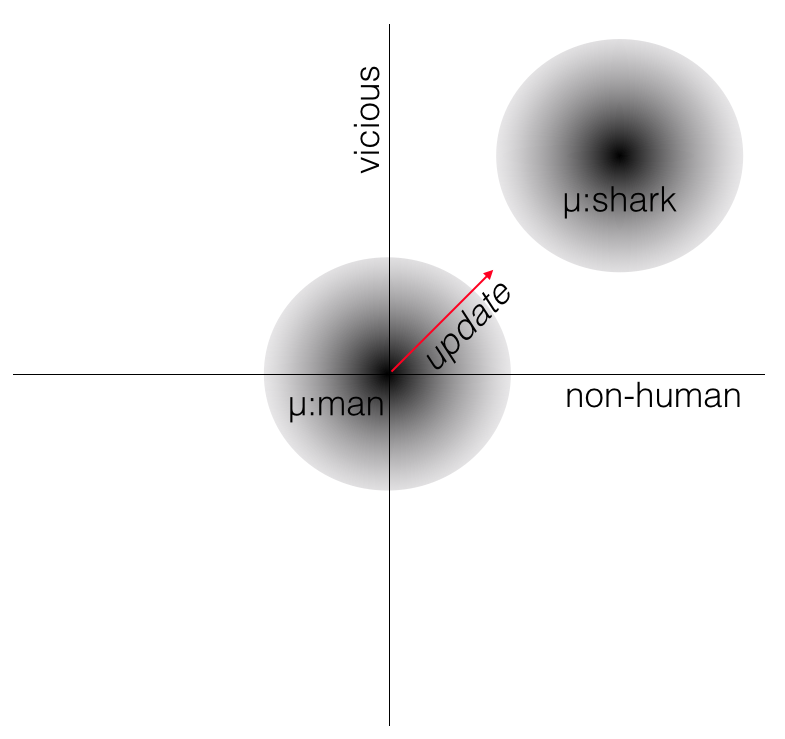
\includegraphics[height=4.5cm]{images/diagram1.png}
		   
		  \caption{Illustration of literal listener $L\protect_0$ given \emph{The man is a shark}, with $\protect\overrightarrow{man}$ = (0,0) and $\protect\overrightarrow{shark}$ = (1,1). $L\protect_0$'s prior is centered at $\protect\overrightarrow{man}$, and is updated towards $\protect\overrightarrow{shark}$.}
		  \label{fig:2d}
		\end{figure}

			% , e.g. $\overrightarrow{\text{temper}}$ for the metaphor \emph{fiery temper}. The points in the distribution represent meanings of \emph{temper} that might not be encoded in its vector. For instance, some points in the distribution might be closer to $\overrightarrow{\text{intense}}$ or $\overrightarrow{\text{unstable}}$. 

		 % of the metaphor, we represent the listener's prior uncertainty over what the subject is like, or equivalently, what point in the space the subject occupies.
			
			% On hearing 

			% Updating one's prior on what time is like, namely the Gaussian centered on $\overrightarrow{\text{time}}$ so that these points have more weight, represents in this model an update regarding one's knowledge about time.

	\paragraph{The semantics}


			% This is unsurprisingly, given that the relational interpretation of $\QLONE$ amounts to the vectorial interpretation, but for a vector space  over the Boolean field, rather than the real field.

		Word embedding spaces allow us to compare the similarity of words (e.g., a noun and an adjective) according to different measures of distance in the space. However, they do not provide a means of categorically determining the compatibility of that adjective and noun, as previous pragmatic models have required (described in Section \ref{rsa}). We observe, however, that the definition of $L_0$ in (\ref{defl0}) only mathematically requires that the semantics $\llbracket \cdot \rrbracket$ be a function $U\to (W\to \mathbb{R})$. We can define such a function as follows, with $\sigma_2$ as a hyperparameter:
		% \vspace{-1.5em}
		\begin{examples}
		
		\item $\llbracket u\rrbracket(w) = P_{\mathcal{N}}(w\vert\mu=E(\textrm{\emph{source}}),\sigma=\sigma_2)$ \label{vect:sem}
		% \overrightarrow{\mathit{predicate_u}}
		\end{examples}

		% However, despite the ``softness'' of a distributional meaning, will find that it is possible to use it to obtain a semantics capable of underlying $\QLONE$, 

		% since the $L_0$ requires only that the semantics be real-valued.



		The value of $\llbracket u\rrbracket(w)$ is a real number which decreases with the Euclidean distance between $u$ and $w$. 
		The advantage of defining the semantics in this way is that both the prior of $L_0$, shown in (\ref{vect:prior}), and the likelihood, in (\ref{vect:sem}), are Gaussian distributions, which allows for a closed form solution of $L_0$, described in \emph{Materials and Methods}. 
		% As with the definition of the prior in (\ref{vect:prior}), the semantics introduces a hyperparameter, namely $\sigma_2$.

	\paragraph{Projections} 

		\begin{figure}
		\centering
			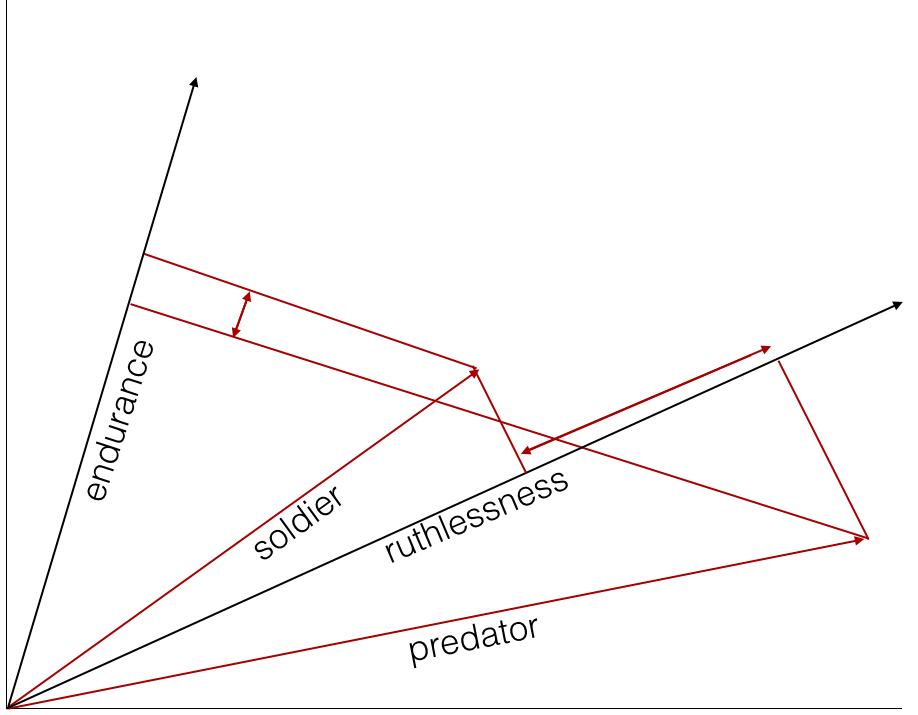
\includegraphics[height=4.5cm]{images/diagram2.png}
			\caption{In this hand-constructed 2D example, vectors for $\protect\overrightarrow{soldier}$ and $\protect\overrightarrow{predator}$ are projected onto subspaces given by $\protect\overrightarrow{endurance}$ and $\protect\overrightarrow{ruthlessness}$. Soldiers have greater endurance than predators, while predators are more ruthless.}
			% In this 2D example, the vectors for \emph{endurance} and \emph{ruthlessness} each parametrize a projection mapping all the points in the space (such as \emph{Jane} and \emph{John}) to new points. These new points can be thought of as the positions of \emph{John}, \emph{Jane} and so on in a new space which cares only about the position of the points with respect to $\protect\overrightarrow{endurance}$ or $\protect\overrightarrow{ruthlessness}$.
			\label{fig:1}
		\end{figure}
		% Since, in a distributional setting, the axes of a world state vector do not neatly correspond to its attributes\footnote{If our space was formed by a basis of co-occurrence vectors, each word would be a dimension, but this is not the case in typical word embedding spaces, the dimensions of which are much fewer than the size of the vocabulary.}, our distributional  cannot simply be a projection along an axis. 

		Finally, we need to supply a notion of a projection function $q$ that is defined on our vector space, and to specify a set $Q$ of such projections. 
		For this, we use linear projections
		% \footnote{To see why this is the natural analogue of the projection functions used in the set-theoretic interpretation of $\QLONE$, note that when viewed as vectors in a vector space over the Boolean field, projection functions are precisely linear projections. Alternatively, note that in either case, projections $q$ are idempotent maps $(W\to W)$.} 
		along a vector (or hyperplane) $\overrightarrow{v}$ 
		% This is a linear transformation from $W$ to the subspace given by $\overrightarrow{v}$, 
		capturing the degree to which each $\overrightarrow{w}$ extends along $\overrightarrow{v}$, ignoring orthogonal dimensions. Geometrically, this amounts to dropping a line from an input vector $\overrightarrow{w}$ at a right angle onto $\overrightarrow{u}$, as depicted in figure \ref{fig:1}. These projections exploit the linear structure of the word embedding space \cite{pennington2014glove}, though see \cite{linzen2016issues,finley2017analogies} for potential caveats.

			% Alternatively, note that 
				% Put another way, the definition of a projection on an object $X$ as an idempotent morphism $X\to X$, generalizes both cases. 
				% ok yes this is deeply unnecessary


				% World states and word denotations in  RSA, as described in (\cite{kao}), can already be understood as vectors over the set of two elements, \{0,1\}, or equivalently as relations between the subject and predicate. (For instance, suppose the meaning of \emph{shark} is $<$vicious=True,aquatic=False$>$. This can be rewritten as the vector $<$1,0$>$.) The intuition behind our model is to generalize QUD RSA to a vector space over the reals.
		% As in the set-theoretic interpretation, w
		In practice, we restrict ourselves to projections along a vector, rather than a larger subspace. 
		% However, we no longer have an obvious set of projections $Q$, corresponding to an explicit set of properties $P$. This is because the basis vectors of a word embedding space such as GloVe or Word2Vec do not correspond to easily interpretable attributes of the words in the space.
		To obtain a set $Q$ of projections, we first note that since word meanings are vectors in $W$, any word parametrizes a linear projection $q$. For instance, we can think of the word \emph{vicious} as defining a \emph{viciousness} projection, which measures how far other points in the space fall along $\overrightarrow{\mathit{vicious}}$. 
		We choose $Q$ as a set of gradable adjectives, so that the projection of a noun onto $\overrightarrow{v}$ amounts to asking: to what extent does the noun have property $v$? 
		Figure \ref{l1heatmaps} provides a visualization of the $\QLONE$ posterior in a simple two-dimensional case corresponding to the example discussed in section \ref{rsa}.


	% \boolean{singlecolumn}
	\begin{figure}
		\hspace{4em}
		\begin{subfigure}{0.3\textwidth}
			\begin{center}

			\setlength\extrarowheight{-10pt}
			\renewcommand{\arraystretch}{0.1}
			\begin{tabular}{ c | c | c  }
			 \tiny $\protect\QLONE$ adjectives & \tiny BASELINE adjectives & \tiny Metaphor \\ 
			\hline
			 % cell4 & cell5 & cell6 \\ 
			 % $\protect\QLONE$ adjectives & BASELINE adjectives & metaphor \\
			\tiny undistorted, faceless & \tiny wolfish, pitiless & \tiny cut-throat competition\\
			\tiny euphoric, giddy & \tiny despondent, chagrined & \tiny deflated emotions\\
			\tiny greater, moral & \tiny alarming, impoverished & \tiny deeper poverty\\
			\tiny traditional, fresh & \tiny homemade, organizational & \tiny corporate pie\\
			\tiny imminent, speculative & \tiny recessionary, substantial & \tiny economic meltdown\\
			\tiny evil, suicidal & \tiny angry, nasty & \tiny blind hate\\
			\tiny stellar, untold & \tiny humiliating, regional & \tiny economic heap\\
			\tiny unbearable, mental & \tiny afflicted, worse & \tiny debilitating poverty\\
			\tiny bipartisan, anti & \tiny political, affordable & \tiny economic prescription\\
			\tiny quiet, idyllic & \tiny important, everlasting & \tiny deserted friendship\\
			\tiny beautiful, particular & \tiny fearful, sincere & \tiny blue feelings\\
			\tiny unproductive, crummy & \tiny ungodly, undoable & \tiny backbreaking rent\\
			\tiny dangerous, possible & \tiny alleged, guilty & \tiny criminal path\\
			\tiny cynical, vulgar & \tiny lustful, insatiable & \tiny dirty desires\\
			\tiny difficult, obvious & \tiny preliminary, analytical & \tiny deep analysis\\
			\tiny easy, traditional & \tiny possible, social & \tiny economic pie\\
			\tiny successive, miserable & \tiny fiscal, brutal & \tiny crushing unemployment\\
			\tiny wrong, new & \tiny warmer, appropriate & \tiny cold justice\\
			\tiny refreshing, copious & \tiny unopened, divine & \tiny bottled passion\\
			\tiny awash, treacherous & \tiny undulating, unprecedented & \tiny crisscrossed chaos\\
			\tiny jubilant, galvanized & \tiny buoyant, wobbly & \tiny deflated pride\\
			\tiny desirable, modest & \tiny residential, fragile & \tiny durable middle-class\\
			\tiny amusing, cynical & \tiny nasty, afraid & \tiny biting look\\
			\tiny recent, likely & \tiny slight, annual & \tiny economic rise\\
			\tiny enduring, rich & \tiny afflicted, global & \tiny deep poverty\\
			\tiny gifted, renowned & \tiny illiterate, national & \tiny blind elite\\
			\tiny federal, necessary & \tiny southern, aggressive & \tiny economic force\\
			\tiny cyclical, breakneck & \tiny zippy, sluggish & \tiny economic laggard\\
			\tiny immense, intellectual & \tiny overall, analogous & \tiny economic sphere\\
			\tiny precarious, creaking & \tiny adequate, prolonged & \tiny collapsing health\\
			\tiny stale, unrealistic & \tiny wobbly, metaphorical & \tiny deflated meaning\\
			\tiny optimal, budgetary & \tiny potential, adequate & \tiny balanced growth\\
			\tiny entrepreneurial, greater & \tiny agile, possible & \tiny economic mobility\\
			\tiny wicked, dishonest & \tiny virtuous, righteous & \tiny dirty deeds\\
			\tiny cultural, genuine & \tiny astonishing, parliamentary & \tiny democratic vitality\\
			\tiny rewarding, excess & \tiny dry, lavish & \tiny draining expense\\
			\tiny vibrant, medieval & \tiny worse, grotesque & \tiny economic tapestry\\
			\tiny relentless, debilitating & \tiny battered, periodic & \tiny crushing cycle\\
			\tiny conquering, immense & \tiny embarrassing, overwhelming & \tiny crushing difficulty\\
			\tiny academic, practical & \tiny advanced, recent & \tiny economic medicine\\
			\tiny pessimistic, bleak & \tiny worried, serious & \tiny clouded future\\
			\tiny ambitious, vibrant & \tiny strategic, postwar & \tiny economic revitalization\\
			\tiny accidental, divergent & \tiny unspoken, intolerable & \tiny colliding contradiction\\
			\tiny appalling, wretched & \tiny alarming, inhuman & \tiny dehumanizing poverty\\
			\tiny overblown, depressing & \tiny bizarre, depressed & \tiny deflated joke\\
			\tiny alone, unclear & \tiny male, additional & \tiny dead money\\
			\tiny enduring, evident & \tiny homogeneous, big & \tiny deep inequality\\
			\tiny supreme, founding & \tiny constitutional, socialist & \tiny dissolved time\\
			\tiny longstanding, unshakeable & \tiny baneful, underlying & \tiny deep-rooted belief\\
			\tiny ambitious, innovative & \tiny outspoken, risky & \tiny aggressive program\\
			\tiny unchecked, continual & \tiny phenomenal, zippy & \tiny breakneck expansion\\
			\tiny rampant, worsening & \tiny acute, fatal & \tiny chronic poverty\\
			\tiny immediate, immense & \tiny atomic, illegal & \tiny economic destruction\\
			\tiny unable, wrong & \tiny heavy, anxious & \tiny broken hope\\
			\tiny internal, sustained & \tiny neurological, apparent & \tiny economic muscle\\
			\tiny inherent, legitimate & \tiny ancient, glaring & \tiny cultural impediment\\
			\tiny ideological, fiscal & \tiny philosophical, administrative & \tiny academic gap\\
			\tiny good, higher & \tiny poor, efficient & \tiny durable class\\
			\tiny worsening, prevalent & \tiny adverse, global & \tiny acute poverty\\
			\tiny successive, heartbreaking & \tiny aggravated, gigantic & \tiny crushing neglect\\
			\tiny unrelenting, magnificent & \tiny windy, torrid & \tiny blazing desolation\\
			\tiny moral, secular & \tiny parliamentary, flexible & \tiny civic fabric\\
			\tiny interactive, competitive & \tiny nonlinear, real & \tiny dynamic company\\
			\tiny principled, definite & \tiny lasting, flexible & \tiny clear-cut solution\\
			\tiny subsidized, costly & \tiny senior, insolvent & \tiny burdened service\\
			\tiny unsustainable, voluminous & \tiny macroeconomic, insufficient & \tiny ballooning expenditure\\
			\tiny lonely, idyllic & \tiny monogamous, featureless & \tiny deserted relationships\\
			\tiny disoriented, contorted & \tiny unexplored, undulating & \tiny choked gullies\\
			\tiny conquering, heartbreaking & \tiny appalling, gigantic & \tiny crushing misery\\
			\tiny dramatic, depressing & \tiny recent, greater & \tiny economic slide\\
			\tiny quiet, nondescript & \tiny forlorn, patterned & \tiny blue obscurity\\
			\tiny foreseeable, pessimistic & \tiny windless, worrisome & \tiny cloudy prospect\\
			\tiny pervasive, debilitating & \tiny addictive, corporate & \tiny corrosive corruption\\
			\tiny widespread, alarming & \tiny abject, escalating & \tiny acute ignorance\\
			\tiny flamboyant, humorous & \tiny multicolored, garish & \tiny colorful personality\\
			\tiny certain, other & \tiny painful, huge & \tiny deep rank\\
			\tiny minor, whole & \tiny good, numerous & \tiny broken melody\\
			\tiny optimistic, generous & \tiny national, ambitious & \tiny compassionate budget\\
			\tiny provocative, unflattering & \tiny memorable, charming & \tiny colorful remark\\
			\tiny feudal, authoritarian & \tiny great, aristocratic & \tiny backward tradition\\
			\tiny civil, disastrous & \tiny sluggish, allied & \tiny economic battle\\
			\tiny consequent, structural & \tiny apparent, freshwater & \tiny ecological collapse\\
			\tiny terrible, oppressive & \tiny absolute, innate & \tiny crushing ignorance\\
			\tiny potential, tremendous & \tiny ready, mild & \tiny big weakness\\
			\tiny unbearable, nagging & \tiny escalating, playful & \tiny crippling awkwardness\\
			\tiny impoverished, prone & \tiny parallel, important & \tiny backward area\\
			\tiny scientific, theoretical & \tiny potential, advanced & \tiny economic field\\
			\tiny economic, ongoing & \tiny bilateral, unprecedented & \tiny deepening crisis\\
			\tiny succinct, emphatic & \tiny goddamned, possible & \tiny clear-cut answer\\
			\tiny spiritual, immense & \tiny otherworldly, heavy & \tiny deep solitude\\
			\tiny intelligent, creative & \tiny narcissistic, aggressive & \tiny dynamic personality\\
			\tiny naive, suicidal & \tiny poor, bald & \tiny blind optimism\\
			\tiny usual, strange & \tiny wet, unlikely & \tiny cold appearance\\
			\tiny enduring, emotional & \tiny aesthetic, newfound & \tiny cultural strength\\
			\tiny bleak, glum & \tiny ghastly, enduring & \tiny dim reminder\\
			\tiny bittersweet, unimaginable & \tiny salty, baked & \tiny delicious agony\\
			\tiny crippling, debilitating & \tiny afflicted, nationwide & \tiny crushing hunger\\
			\tiny productive, scarce & \tiny active, hydrochloric & \tiny concentrated poverty\\
			\tiny romantic, pure & \tiny youthful, pale & \tiny dark passion\\
			\tiny aware, direct & \tiny administrative, unable & \tiny clear responsibility\\
			\tiny pessimistic, bleak & \tiny enticing, heightened & \tiny dimmed prospect\\
			\tiny longstanding, generational & \tiny ingrown, hallowed & \tiny deep-rooted tradition\\
			\tiny sleazy, seedy & \tiny new, formal & \tiny dodgy bar\\
			\tiny sacred, holy & \tiny yellow, kindred & \tiny burning soul\\
			\tiny timeless, immortal & \tiny rejuvenated, mellow & \tiny ageless rhythms\\
			\tiny serene, otherworldly & \tiny overgrown, lyrical & \tiny desolate beauty\\
			\tiny disastrous, debilitating & \tiny fierce, avenging & \tiny crushing effect\\
			\tiny wasteful, unsustainable & \tiny lifeless, tough & \tiny bloated spending\\
			\tiny thriving, vibrant & \tiny pigtailed, unraveled & \tiny blossoming industry\\
			 
			\end{tabular}
			\end{center}
		\end{subfigure}\begin{subfigure}{0.5\textwidth}
			% 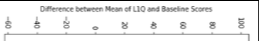
\includegraphics[width=4.5cm]{images/top.png}\\ 
			\vspace*{-1.3cm}\hspace{6em}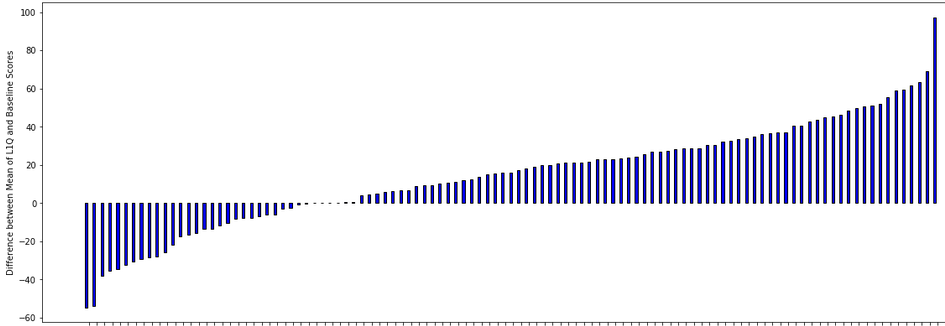
\includegraphics[width=18.9cm,height=6.5cm,angle=270]{images/resultsbarplot.png}
		\end{subfigure}
			\caption{The 109 metaphors used in the experiment, and baseline and $\protect\QLONE$ interpretations. Bar positions indicate difference between judgments of $\QLONE$ and baseline proposals, averaged across participants and across both proposals of each model. Bars right of center indicate a preference for the pragmatic model, showing that for roughly 75\% of the metaphors, the $\protect\QLONE$ interpretation is preferred.
			}
			\label{fig:barplot}
		\end{figure}


	\begin{figure*}

	\centering

	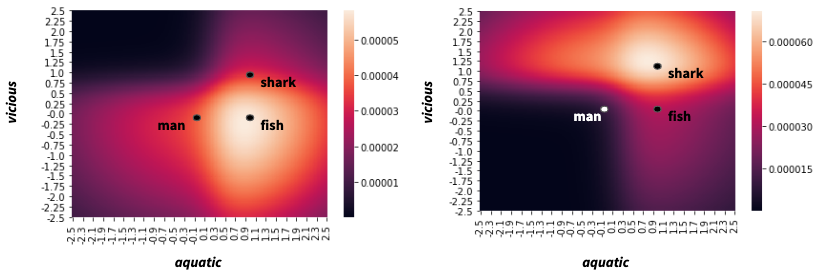
\includegraphics[width=\textwidth]{images/bothheatmaps.png}

	% \begin{subfigure}{0.5\textwidth}

	% \centering

	% 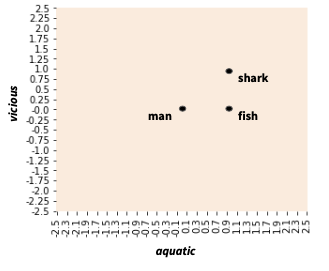
\includegraphics[width=0.85\textwidth]{images/denotations.png}

	% \end{subfigure}\hfill\begin{subfigure}{0.5\textwidth}

	% \centering

	% 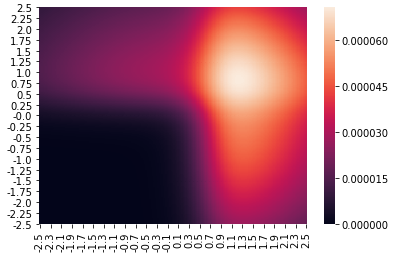
\includegraphics[width=\textwidth]{images/discretel1heatmap.png}

	% \end{subfigure}

	\caption{Heatmaps visualizing the inferred $\protect\QLONE$ marginal posterior over states in a two-dimensional case given \emph{fish} (left) and \emph{shark} (right), with $U = \{$\emph{man}, \emph{shark}, \emph{fish}$\}$, hand-chosen denotations overlaid, and $\protect\sigma\protect_1=5.0, \protect\sigma\protect_2=0.5$. $Q$ consists of two projections, one along the x-axis (\emph{aquatic}) and one along the y-axis (\emph{vicious}).}

	% Comparison between the $\protect\QLONE$ posterior under our inference algorithm (left) and under the true posterior (right), which is calculable in this two dimensional case (up to discretization of the space).

	\label{l1heatmaps}

	\end{figure*}
 





		% To compute the joint posterior over $W$ and $Q$, we first compute the conditional posterior $P(w|q,u)$ for each $q\in Q$, and then determine the marginal posterior on $Q$, $P(Q)$  HOW THO? 

		

		% fixing a particular projection $q$, we can compute the conditional probability of $w$ 
			% for an orthonomal basis of $W$ including $q$, the mean and variance of this posterior is the same as the prior in every dimension except $q$. 
			% 	In the single dimension of interest, we approximate the conditional posterior by performing gradient descent to find the mean of the posterior, and discretizing the now one-dimensional prior. 





	% $L_1$ is defined as follows, where P$_{QUD}$ represents the prior on QUDs. As discussed below, we can either have this be a continuous distribution over hyperplanes corresponding to projection functions, or a discrete distribution of hyperplanes corresponding to a set of n-tuples of words. In either case, we assume it is a uniform distribution:
	% \begin{examples}
	% \item $L_1(w,q\vert u) \propto S_1(u\vert w,q) P_{\mathcal{N}}(w\vert\mu=subject,\sigma=\sigma_1)*P_{QUD}(q)$
	% \end{examples}
	% While we were able to use analytic methods to derive the $L_0$ and $S_1$ posteriors, we cannot do so for the $L_1$. Instead, we must use an approximate inference method. We try two different inference algorithms, Hamiltonian Monte Carlo (\cite{neal2011mcmc}), a brand of Markov Chain Monte Carlo inference algorithm which makes use of gradient information to move from one sample to the next, and Variational Mean Field inference (see \cite{blei2017variational}), an optimization based inference algorithm. In our first experiment we use the former, while we make use of the latter in our second, on account of its speed.

	% Variational Inference (VI) greatly increases efficiency over other inference methods, at the cost of requiring gradients for the $S_1$ and the functions the $S_1$ calls. Fortunately, it is possible for us to calculate these gradients, using automatic differentiation.

	% $L_1$ performs joint inference over QUDs and worlds. While the nature of the prior over worlds has already been discussed, two variants of $L_1$ are possible, as regards to prior on QUDs. The first is to have a categorical distribution over a set of projection hyperplanes (QUDs), for example those corresponding to n-tuples of words, according to the pretrained embedding. The output of our inference then gives us a categorical distribution over QUDs, corresponding to words (as well as a continuous distribution over worlds). 

	% The second variant is to have the QUD be a continuous variable. As a result of the way the projection is defined, only the angle and not the magnitude of the projection hyperplane matters. As such, we can have a uniform prior over unit hyperplanes. We will refer to these as two models as the Categorical and Non-Categorical $L_1$, respectively.

	% The advantage of the Categorical $L_1$ is that we can choose a particular set of QUDs, for instance, the vectors corresponding to a given set of words, and weight this prior according to the frequency of these words. This allows us to supply our model with a set of possible QUDs, and have it return a categorical distribution over them, as the $L_1$ QUD posterior.

	% The Non-Categorical model, on the other hand, has the contrasting benefit that no set of possible QUDs need be provided to the model. Furthermore, the use of Hamiltonian dynamics for performing the joint inference results in much faster performance. However, the Non-Categorical model yields significantly less stable results, and as such, we use only the Categorical model in our experimentation.
% \vspace{2em}
\paragraph{Interpreting the output of $\protect\QLONE$}

	The \emph{Materials and Methods} describes how to calculate the interpretation of a metaphor $u$ given these assumptions. In particular, it shows how to compute $\QLONE(w,q|u)$, the joint distribution over states and projections after hearing a metaphor $u$. Unlike points $\overrightarrow{w}\in W$, projections $\overrightarrow{q}\in Q$ are readily interpretable, since they correspond to adjectives, describing the aspect of the metaphorical adjective or predicate that is inferred to be relevant.
		% Each $q\in Q$ corresponds to an adjective, describing the aspect of the metaphorical adjective or predicate that the speaker considers relevant. 
	For this reason, we use the marginal posterior over $Q$ to generate predictions from the model. The top two $\QLONE$ marginal posterior projections $\overrightarrow{q}$ for each metaphor, which we use in our experiment, are shown in the leftmost column of Figure \ref{fig:barplot}. 

	% We convert this into an interpretable prediction by selecting the adjectives $q\in Q$ which have high probability under the marginal posterior distribution over $Q$ as interpretations of the metaphor.




\section{Experimental Evaluation} \label{exp}

	In order to evaluate whether pragmatic reasoning results in metaphor interpretations that better capture human judgments, we designed an experiment comparing $\QLONE$ interpretations of metaphors to a baseline model which uses word embeddings but no pragmatic reasoning.


	\subsection*{Experimental Design}

		In the experiment, each participant was shown a series of 12 adjectival metaphors, selected randomly from a total of 109. For each metaphor, they were asked to rate four candidate interpretations of the metaphor on a slider bar. These four candidate interpretations consist of the best and second best adjective generated by $\QLONE$, and similarly for a baseline model. The baseline model selects adjectives without pragmatic reasoning, using a standard procedure from the word embeddings literature (see \emph{Materials and Methods}). An example is shown in Figure \ref{fig:slide}.


	
	
		% (the variances of the Gaussians used in the prior and semantics respectively). 

	\subsection*{Analysis}
	% \paragraph{Analysis}

		The results, shown in Figure \ref{fig:barplot}, were analyzed using mixed-effects models with random slopes and intercepts for items and participants. Participants rated four interpretations for each metaphor: the best and second-best interpretations, as output by each of the target and baseline models. Participants rated the target interpretations significantly higher than the baseline interpretations ($\beta$=13.8, $t$=5.3, p$<10^{-7}$) in a combined analysis. The results were similar when the best target interpretations were compared to the best baseline interpretations ($\beta$=16.4, $t$=4.8, p$<10^{-5}$) and when the second-best interpretations were compared ($\beta$=11.1, $t$=3.2, p$<$0.005).

		% Using the same mixed-effects model, we further find a significant preference for the $\QLONE$ best adjective over the second best adjective ($\beta$=, $t$=, p$<$), indicating that TODO


		
		% We ran a linear mixed effects model, predicting slider rating from baseline vs. $L_1$ metaphor, with by-metaphor and by-participant random intercepts. We find a significant correlation

			% As can be seen in Figure \ref{resultsbar}, there is a lot of variation in the average quality of proposed adjectives across both models, between metaphors. For the baseline model, we note that there is a subset of metaphors for which the baseline will perform well, as discussed in section (\ref{task1id}). These are metaphors where good projections $q$ are such that the subject and predicate are close when projected along $q$. In these cases, averaging the subject and predicate will generally give rise to a good interpretation. 
\section{Discussion} \label{conc} 

	We have shown that it is possible to scale Bayesian pragmatic reasoning to distributional semantics, and using this to obtain a model of metaphor interpretation. Our evaluation, the first open-domain evaluation of a Bayesian model of pragmatic language interpretation, indicates that the principles of pragmatic reasoning continue to operate at this scale, and are key to obtaining human-like interpretations of metaphors. We see this as an important step towards a cognitively accurate and computationally tractable model of pragmatic language interpretation and production in general.

% \section*{Guide to using this template on Overleaf}


% If you have a question while using this template on Overleaf, please use the help menu (``?'') on the top bar to search for \href{https://www.overleaf.com/help}{help and tutorials}. You can also \href{https://www.overleaf.com/contact}{contact the Overleaf support team} at any time with specific questions about your manuscript or feedback on the template.




% \paragraph*{3D Figures}

% Supply a composable U3D or PRC file so that it may be edited and composed. Authors may submit a PDF file but please note it will be published in raw format and will not be edited or composed.


\matmethods{
% Please describe your materials and methods here. This can be more than one paragraph, and may contain subsections and equations as required. Authors should include a statement in the methods section describing how readers will be able to access the data in the paper. 

% \paragraph{$\mathbf{\QLONE}$ Model}

% To derive predictions from $\QLONE$, five things must be provided: a set $W$ of states, a set $U$ of utterances, a set $Q$ of projections, a prior $P_L$ representing the listener's uncertainty over $W$, and a semantics $\llbracket\cdot\rrbracket$. (We assume throughout that the prior $P_{L_Q}$ over $Q$ is uniform.) Jointly, we say that these determine an \emph{interpretation} of $\QLONE$. 

% 		One possible interpretation, similar to what is provided by \cite{kao}, treats points in the state space $W$ as n-tuples of truth values, corresponding to Boolean properties $w\subset P$.
% 		% with a function $E:U\to \mathcal{P}(P)$ mapping utterances to sets of properties. 
% 		% We refer to this as a \emph{set theoretic} interpretation of $\QLONE$. 
% 		We give a very simple example below, for $P = \{\textrm{vicious}, \textrm{non-human} \}$:

% 		\begin{itemize}
% 		% \item $W = \{(\textrm{vicious}=T,\textrm{non-human}=T), \\ (\textrm{vicious}=T,\textrm{non-human}=F),\\ (\textrm{vicious}=F,\textrm{non-human}=T),\\ (\textrm{vicious}=F,\textrm{non-human}=F) \}$
% 		% \item $W = \{ \{\textrm{vicious}, \textrm{non-human}\}, \{\textrm{vicious}\}, \{\textrm{non-human}\}, \{\},   \}$
% 		\item $P_L = \{(\textrm{vicious}=T,\textrm{non-human}=T) : 0.075, \\(\textrm{vicious}=T,\textrm{non-human}=F) : 0.675,\\ (\textrm{vicious}=F,\textrm{non-human}=T) : 0.025, \\(\textrm{vicious}=F,\textrm{non-human}=F): 0.225\}$
% 		% \item $W = \{ \{\textrm{vicious}, \textrm{non-human} \}, \{\textrm{vicious} \}, \{\textrm{non-human} \}, \{\},   \}$
% 		\item $U = \{\textrm{\emph{shark}}, \textrm{\emph{silence}}\}$
% 		% \item $\llbracket\cdot\rrbracket$
% 		\item $Q = \{q_{vicious} = \lambda (x,y):x, \quad q_{non-human} = \lambda (x,y):y) $ 
% 		\end{itemize}

% 		We assume a semantics $\llbracket\cdot\rrbracket$ in which \emph{shark} is compatible only with $(\textrm{vicious}, \textrm{non-human})$, and \emph{silence} is compatible with every state. Note that the projections map each tuple to its value at a single property. 

\subsection*{Model inference} \label{technicaloverview}


	% Calculating the posterior of $\QLONE$ given an utterance $u$ is far more difficult in the vectorial interpretation than the set-theoretic one. 
	We employ a mix of analytic and approximate methods to compute the $\QLONE$ distribution. We first present the approach for computing $L_0$ and $S_1$ posteriors, which can be done analytically, and then present the approximate inference algorithm for $\QLONE$.
	% \footnote{Inference for all our models is implemented in Tensorflow, and will be made publicly available.} 
	The implementation, written in TensorFlow, will be made publicly available.

	% While the general format of our model is analogous to previous models in the RSA paradigm, the vectorial setting produces a number of challenges which require novel solutions.

	% Moreover, previous implementations of RSA have employed prior distributions for both the speaker and listener with finite support. As a result, it is possible in standard RSA to perform exact inference for the $L_0$, $S_1$ and $L_1$. By contrast, our prior is a Gaussian and as such cannot be computed via exact inference, due to the need to calculate a normalizing term which sums (or rather integrates) over an infinite set. 
	% Furthermore, nesting causes approximate inference in the form of Markov Chain Monte Carlo to be unstable (see \cite{rainforth2016pitfalls}).
	% We therefore compute the $L_0$ and $S_1$ posteriors analytically, and use perform appromixate inference only at the $L_1$ level. We now describe how each of $L_0$, $S_1$ and $L_1$ is computed.
% \paragraph{L\textsubscript{0} Inference}

	\paragraph{$\mathbf{L_0}$ Inference}
	The vector interpretation of $L_0$ is illustrated in Figure \ref{fig:2d}, where a ball, corresponding to the prior, is moved in the direction of the point corresponding to the perceived utterance. To calculate $L_0$ analytically, we make use of Gaussian conjugacy. When the prior $P_L$ is defined as in Equation \ref{vect:prior}, and the semantic interpretation is defined as in Equation \ref{vect:sem}, then conjugacy implies that the listener posterior is given by:

	 \begin{examples}
	\item $L_0(w|u)=P_{\mathcal{N}}(w\vert\mu\! \! =\! \! \frac{\sigma_1^2 \sigma_2^2}{\sigma_1^2+\sigma_2^2}(\frac{{\textrm{\emph{E(target)}}}}{\sigma_1^2}+\frac{{\textrm{\emph{E(source)}}}}{\sigma_2^2}), \sigma \! \!=\! \! \frac{\sigma_1^2 \sigma_2^2}{\sigma_1^2+\sigma_2^2})$  \label{eq:L0-inference}
	 \end{examples}





	% This is the property that a distribution of the form $P_{\mathcal{N}}(w\vert\mu=subject,\sigma=\sigma_1)P_{\mathcal{N}}(w\vert\mu=u,\sigma=\sigma_2)$



	% Recall that $L_0$ is defined as follows, where \emph{subject} is the word being predicated (e.g. ``lawyer'' in ``The lawyer is a shark''):



	% \begin{examples}

	% \item $L_0(w\vert u) \propto P_{\mathcal{N}}(w\vert\mu=subject,\sigma=\sigma_1)P_{\mathcal{N}}(w\vert\mu=u,\sigma=\sigma_2)$ \label{term}

	% e^f$ * e$^\mu$ \label{term}

	% \end{examples}

	% The left hand term represents the prior on the world state, and the right hand term represents the observation. By the self conjugacy of Gaussians, (\ref{term}) can be reduced analytically to a single Gaussian.

	% 	 citation?
% \paragraph{S\textsubscript{1} Inference}
\paragraph{$\mathbf{S_1}$ Inference}
		The speaker is defined by Equation \ref{defs0}, which in the continuous case can be rewritten as:
		\begin{examples}
		\item $S_1(u\vert w,q) \propto \int_{w'} \delta_{q(w)=q(w')} \cdot L_0(w'\vert u)$
		\end{examples}
		Here $q(w)$ is the projection of state $\overrightarrow{w}$ onto the subspace spanned by projection vector $\overrightarrow{q}$. This integral computes the marginal probability of all states that are projected to the same location as $\overrightarrow{w}$ along $\overrightarrow{q}$. From Equation \ref{eq:L0-inference}, $L_0(\cdot \vert u)$ is a normally distributed random variable, and therefore the projection of this random variable onto a linear subspace is also normally distributed, providing a closed-form solution to $S_1$.

		% We refer to the hyperplane which parametrizes the QUD projection as $\overrightarrow{\text{q}}$, and abuse notation by having q(v) denote the vector resulting from a projection of v along q. Note that q(v) could either be represented in the dimensionality of the original space or the projection subspace. We will assume the former, so that if v $\in$ {\rm I\!R}$^n$, q(v) $\in$ {\rm I\!R}$^n$. Then our $S_1$ is almost identical to the plain QUD RSA model:



		% \begin{examples}

		% \item U(u,w,q) = $\log(\int_{w'} \delta_{q(w)=q(w')} * L_0(w'\vert u))$

		% \item S$_1(u\vert w,q) \propto e^{U(u,w,q)}$

		% \end{examples}
% \paragraph{L\textsubscript{1} Inference}
\paragraph{$\mathbf{\QLONE}$ Inference}





	



	% \begin{figure}

	% \centering

	% \begin{subfigure}{0.5\textwidth}

	% % \centering

	% 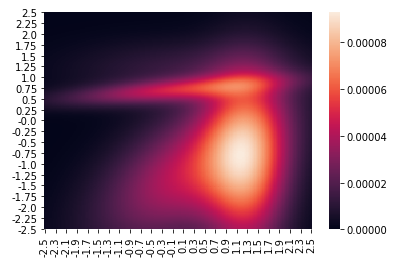
\includegraphics[width=\textwidth]{images/coolmixturel1heatmap.png}

	% \end{subfigure}\hfill\begin{subfigure}{0.5\textwidth}

	% % \centering

	% 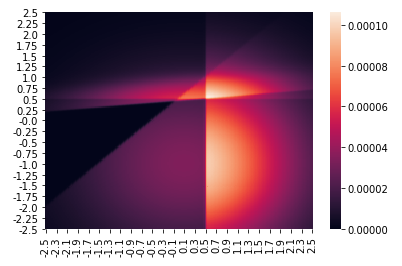
\includegraphics[width=\textwidth]{images/cooldiscretel1heatmap.png}

	% \end{subfigure}

	% \caption{ Comparison between the $\protect\QLONE$ posterior under our inference algorithm (left) and under the true posterior (right), which is calculable in this two dimensional case (up to discretization of the space).}

	% \label{l1heatmaps}

	% \end{figure}



	% caption: 

	% 	heatmaps showing...

	% 	an example of the difference between the $\protect\QLONE$ posterior under our inference algorithm and under the true posterior, in a two dimensional case where a (discretized) exact posterior can be computed exactly.

	% 	this compares our inference algorithm (left) to an exact (discretized) inference in a tractable 2 dimensional case, for the metaphor: BLAH 

	% 	with the following hand-specified word embeddings.





	% caption:

	% 	heatmaps showing the l1 inference. 

	% 		scalar implicature means that...

	% We devise the following approximate inference algorithm.



	The $L_1$ posterior is a joint distribution over one continuous and one discrete random variable. 
	% Unlike $L_0$, we are unable to use conjugacy to compute it analytically.
	Because of the linear structure of the problem, we are able to devise a near-exact inference algorithm for the marginal distribution over projections in $Q$, derived as follows:



	%\footnote{We verify the correctness of this algorithm in the 2 dimensional case by comparison to the exact posterior, which is calculable (up to discretization of the prior) in 2 dimensions.}



		% Moreover, we find that Mean Field Variational Inference  CITATION is not well suited

		% 	since the posterior is non-Gaussian (see figure \ref{l1heatmaps}).



	% \begin{align}

	% L_1(w,q | u) &= \frac{P(w)P(q)S_1(u|w,q)}{\sum_{q'} \int_{w'} P(w')P(q')S_1(u|w',q')} \\

	% &= \frac{P(w)P(q)S_1(u|w,q)}{K} 

	% \end{align}









	% To compute the marginal distribution over QUDs:



	 \begin{align}
	 \begin{split}
	&L_1(q | u) = \int_{\mathbb{R}^n}L_1(w,q | u) dw = \frac{1}{K}P_{L_Q}(q) \int_{\mathbb{R}^n}P_L(w)S_1(u|w,q) dw \\
	&= \frac{1}{K}P_{L_Q}(q) \int_{\mathbb{R}^n}P_L(w_q, w_\bot)S_1(u|w_q,q) dw \\
	% &= \frac{1}{K}P_{L_Q}(q) \int_{\mathbb{R}^n}P_L(w_q) P_L(w_\bot)S_1(u|w_q,q) dw \\
	&= \frac{1}{K}P_{L_Q}(q) \int_{D^\bot}P_L(w_\bot) dw_\bot \int_{D}P_L(w_q) S_1(u|w_q,q) dw_q \\
	&= \frac{1}{K}P_{L_Q}(q)  \int_{D}P_L(w_q) S_1(u|w_q,q) dw_q\nonumber
	\end{split}
	 \end{align}
	



	Here $K$ is a normalizing constant, $\overrightarrow{w}, \overrightarrow{q}\in \mathbb{R}^n$, and $\overrightarrow{w_q}$ is the projection of $\overrightarrow{w}$ onto the vector $\overrightarrow{q}$. $D$ is the subspace of $\mathbb{R}^n$ spanned by the vector $\overrightarrow{q}$, and $D^\bot$ is the orthogonal complement of $D$. 
	The vector $\overrightarrow{w_\bot}$ is the projection of vector $\overrightarrow{w}$ onto the subspace $D^\bot$. The final equation is a one-dimensional integral, and can be computed using a discrete approximation. We use a Gaussian approximation, which easily generalizes to the setting of multi-dimensional projections. The constant $K$ can be found from the constraint $\sum_q L_1(q|u) = 1$.

% \subsection*{Subsection for Method}
% Example text for subsection.



\subsection*{Experiment}

		The aim of our experiment is to determine whether pragmatic reasoning results in better interpretations of metaphors, according to human judgments. We compare against a lesioned model, with a distributional semantics that does not make use of pragmatic reasoning.

		\paragraph{Baseline model}
		Our baseline model is defined as follows: for a given metaphor of the form $(a$ $n)$, we take the mean of the adjective word embedding $E(a)$ and the noun word embedding $E(n)$. The two nearest adjectives $q$ to this mean (measured by cosine distance) are the baseline interpretations for the metaphor. Taking the mean of word vectors is a standard technique for computing phrase and sentence meanings from constituent words \cite{mitchell2010composition,grefenstette2013category,socher2013recursive}, while cosine distance is commonly used to find words with the most similar meaning \cite{pennington2014glove}.



			% relevant literature on vector addition / cosine:
			% 1. https://nlp.stanford.edu/~socherr/EMNLP2013_RNTN.pdf
			% 2. https://arxiv.org/pdf/1311.1539.pdf (section 2.3.1 onward)
			% 3. http://aclweb.org/anthology/E17-1006 (relevant to us)
			% 4. Much cited: https://onlinelibrary.wiley.com/doi/pdf/10.1111/j.1551-6709.2010.01106.x
			% Cosine distance for nearest neighbour:
			% https://nlp.stanford.edu/pubs/glove.pdf
			


	% \begin{figure}
	% 	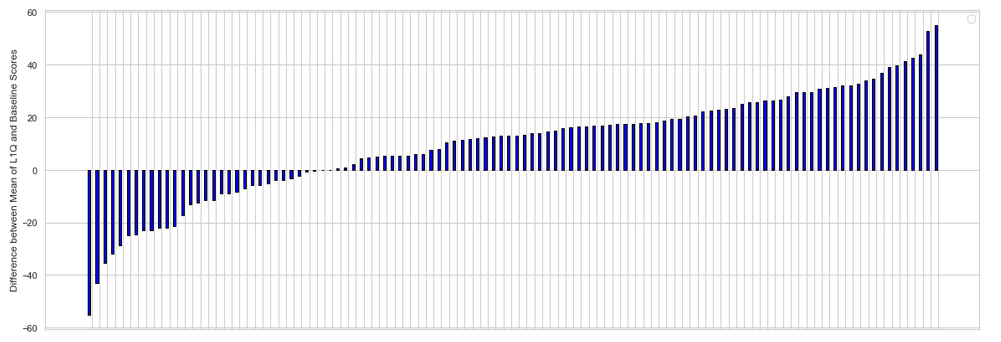
\includegraphics[height=5cm,angle=270,origin=c]{images/comparison1}


	% \end{figure}
	% \begin{figure}
	% 	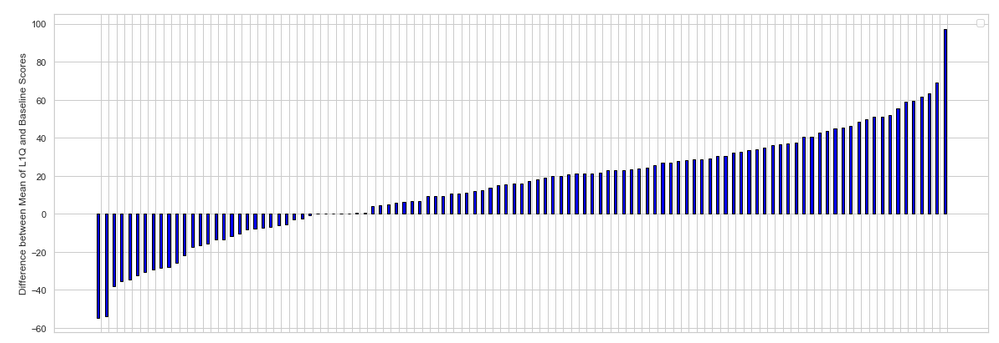
\includegraphics[height=5cm,angle=270,origin=c]{images/comparison2}	
	% \end{figure}

	% \paragraph{$\protect\QLONE$ hyperparameters}
	\paragraph{$\mathbf{\QLONE}$ hyperparameters}

		We use the largest available (300 dimensional) GloVe vectors, as our word embedding $E$. For each Adjective-Noun metaphor $(a$ $n)$, we specify $U$ as a set of 101 alternative utterances, consisting of $a$ and 100 of the nearest adjectives (by cosine distance) to $n$. These adjectives are chosen from the set of the 1425 adjectives with concreteness ranking $>3.0$ in the concreteness corpus of \cite{brysbaert2014concreteness}, to exclude abstract nouns.
		Similarly, we select a set $Q$ of projections corresponding to the hundred closest adjectives to the mean of the subject and predicate (the method of adjective choice in the baseline model), and take $P_{L_Q}$ to be a uniform distribution over $Q$. 

		By tuning on an independent validation set of metaphors, we choose $\sigma_1=\sigma_2=0.1$; all model parameters and features of the architecture were frozen prior to the experiment. Metaphor interpretations are generated by selecting the two projections with highest marginal posterior mass under $\QLONE$. We choose two rather than one since the model tends to distribute most of its probability mass to at least two projections, intuitively reflecting the fact that there is usually more than one good interpretation of a metaphor.

\paragraph{Experimental Methods}

\begin{figure}
\centering
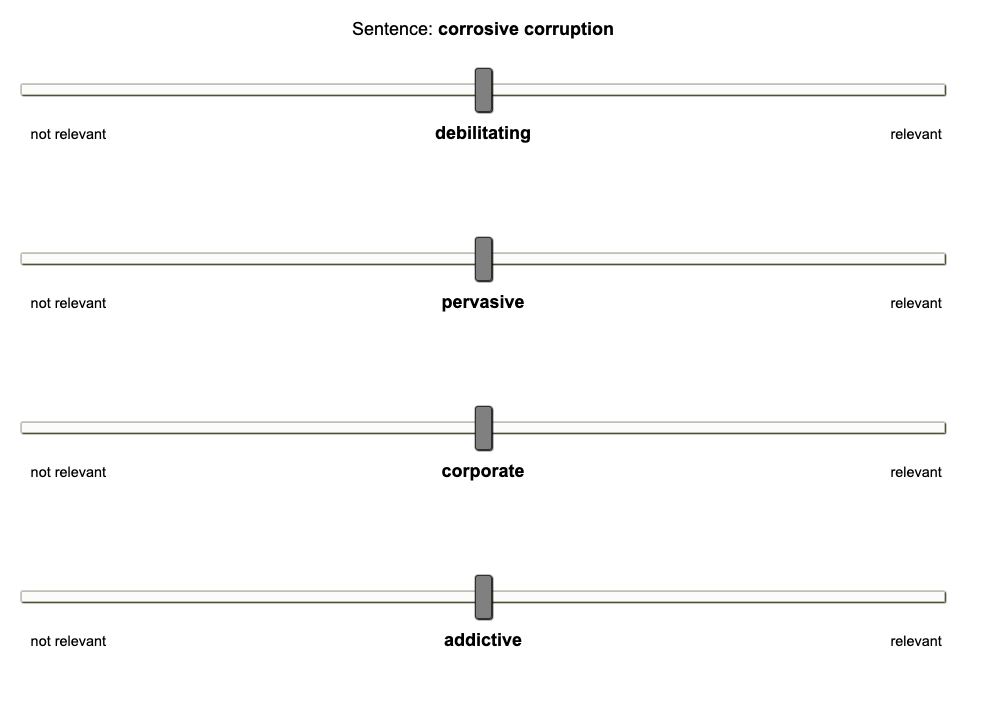
\includegraphics[width=0.45\textwidth]{images/slide.png}
\caption{An item in the experiment. Item order, and order of the 4 candidate adjectives are randomized.}
\label{fig:slide}
\end{figure}

		
		Tsvetkov et al. \cite{tsvetkov2014metaphor} provide a corpus of $\sim$800 AN metaphors, gathered by human annotators, from which we select the least frequent by bigram count (n-gram data from the Corpus of Contemporary American English \cite{davies2011word}) to filter out conventionalized metaphors. Our full set of 109 metaphors is shown in figure \ref{fig:barplot}.
		The experiment was run on Mechanical Turk, with 99 native English speakers. Participants who failed to follow instructions on a test item were excluded, leaving 60 participants (analyses remain significant with all participants included).
		Participants are shown a metaphor, as in figure \ref{fig:slide} and asked to judge how relevant each proposed adjective (here, \emph{debilitating}, \emph{pervasive}, \emph{corporate}, \emph{addictive}) is to the metaphorical meaning of the AN phrase. In a test example, they are told to rate \emph{intense} as relevant to \emph{fiery temper} ``because a fiery temper is an intense temper'' but rate \emph{warm} as irrelevant.

}

\showmatmethods{} % Display the Materials and Methods section

\acknow{Please include your acknowledgments here, set in a single paragraph. Please do not include any acknowledgments in the Supporting Information, or anywhere else in the manuscript.}

% \showacknow{} % Display the acknowledgments section

% Bibliography
\bibliography{metaphor}
\end{document}
